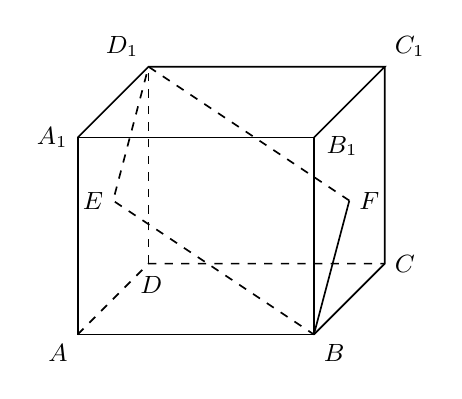
\begin{tikzpicture}[line width=0.6pt, font=\small]
  \coordinate (A) at (0,0);
  \coordinate (B) at (3,0);
  \coordinate (B1) at (3,2.5);
  \coordinate (A1) at (0,2.5);
  \coordinate (D) at (0.9,0.9);
  \coordinate (C) at (3.9,0.9);
  \coordinate (C1) at (3.9,3.4);
  \coordinate (D1) at (0.9,3.4);
  \coordinate (E) at (0.4500000000,1.7000000000);
  \coordinate (F) at (3.4500000000,1.7000000000);
  % front face solid
  \draw (A) -- (B) -- (B1) -- (A1) -- cycle;
  % top face solid
  \draw (A1) -- (D1) -- (C1) -- (B1);
  % right/bottom visible edges solid
  \draw (B) -- (C) -- (C1);
  \draw (B) -- (B1);
  % hidden cube edges dashed
  \draw[dashed] (A) -- (D) -- (C);
  \draw[dashed] (D) -- (D1);
  % quadrilateral BFD1E: BF solid, rest dashed
  \draw (B) -- (F);
  \draw[dashed] (F) -- (D1) -- (E) -- (B);
  % labels
  \node[below left] at (A) {$A$};
  \node[below right] at (B) {$B$};
  \node[right] at (C) {$C$};
  \node[below,xshift=1pt,yshift=-1pt] at (D) {$D$};
  \node[left] at (A1) {$A_{1}$};
  \node[right,xshift=1pt,yshift=-3pt] at (B1) {$B_{1}$};
  \node[above right] at (C1) {$C_{1}$};
  \node[above left] at (D1) {$D_{1}$};
  \node[left] at (E) {$E$};
  \node[right] at (F) {$F$};
\end{tikzpicture}
